\documentclass[11pt,a4paper]{article}

% ----------------------------
% Packages (portable, "beautiful" defaults)
% ----------------------------
\usepackage[a4paper,margin=1in]{geometry}
\usepackage[T1]{fontenc}
\usepackage[utf8]{inputenc}
\usepackage{lmodern}
\IfFileExists{microtype.sty}{\usepackage{microtype}}{} % optional on minimal TeX installs
\usepackage{graphicx}
\usepackage{xcolor}
\usepackage{hyperref}
\IfFileExists{bookmark.sty}{\usepackage{bookmark}}{} % optional
\usepackage{enumitem}
\usepackage{booktabs}
\usepackage{array}
\usepackage{tabularx}
\usepackage{caption}
\IfFileExists{subcaption.sty}{\usepackage{subcaption}}{} % optional
\usepackage{fancyhdr}
\IfFileExists{titlesec.sty}{\usepackage{titlesec}}{} % optional
\usepackage{listings}
\newif\iftcolorboxavailable
\IfFileExists{tcolorbox.sty}{\tcolorboxavailabletrue\usepackage{tcolorbox}}{\tcolorboxavailablefalse}
\newif\iftikzavailable
\IfFileExists{tikz.sty}{\tikzavailabletrue\usepackage{tikz}}{\tikzavailablefalse}
\iftikzavailable
  \usetikzlibrary{positioning}
\fi

% ----------------------------
% Theme: Light Blue & White
% ----------------------------
\definecolor{AccentBlue}{HTML}{2B8CFF}
\definecolor{AccentBlueDark}{HTML}{1F5FB3}
\definecolor{SoftGray}{HTML}{F4F6F9}
\definecolor{TextGray}{HTML}{2B2F36}

\hypersetup{
  colorlinks=true,
  linkcolor=AccentBlueDark,
  urlcolor=AccentBlueDark,
  citecolor=AccentBlueDark,
  pdftitle={Library Management System (C++17) - Report},
  pdfauthor={Muhammad Asif Khan},
  pdfsubject={C++17, Data Structures, Dear ImGui + SFML GUI},
  pdfkeywords={C++17, BST, LinkedList, Queue, ImGui, SFML, CSV}
}

% Headings (use titlesec if available; otherwise default article headings)
\IfFileExists{titlesec.sty}{
  \titleformat{\section}
    {\Large\bfseries\color{AccentBlueDark}}{\thesection}{0.6em}{}
  \titleformat{\subsection}
    {\large\bfseries\color{AccentBlueDark}}{\thesubsection}{0.6em}{}
}{}

% Header/footer
\pagestyle{fancy}
\fancyhf{}
\lhead{\textbf{Library Management System}}
\rhead{\textcolor{AccentBlueDark}{C++17 • Dear ImGui • SFML}}
\cfoot{\thepage}
\renewcommand{\headrulewidth}{0.4pt}
\renewcommand{\footrulewidth}{0pt}

% Lists
\setlist[itemize]{leftmargin=*,topsep=3pt,itemsep=2pt}
\setlist[enumerate]{leftmargin=*,topsep=3pt,itemsep=2pt}

% Code listings (no external deps like minted)
\lstdefinestyle{cpp}{
  language=C++,
  basicstyle=\ttfamily\small,
  keywordstyle=\color{AccentBlueDark}\bfseries,
  commentstyle=\color{gray},
  stringstyle=\color{AccentBlueDark},
  numbers=left,
  numberstyle=\tiny\color{gray},
  stepnumber=1,
  numbersep=8pt,
  frame=single,
  framerule=0.2pt,
  rulecolor=\color{gray!40},
  breaklines=true,
  tabsize=2,
  showstringspaces=false,
  backgroundcolor=\color{SoftGray}
}
\lstset{style=cpp}

% Callout boxes (tcolorbox if available; otherwise fall back to a simple \fcolorbox)
\iftcolorboxavailable
  \newtcolorbox{infobox}[1]{
    colback=SoftGray,
    colframe=AccentBlue,
    coltitle=TextGray,
    title=\textbf{#1},
    boxrule=0.6pt,
    arc=6pt,
    left=10pt,right=10pt,top=8pt,bottom=8pt
  }
\else
  \newenvironment{infobox}[1]{%
    \par\noindent
    \begingroup
    \setlength{\fboxsep}{8pt}%
    \color{TextGray}%
    \fcolorbox{AccentBlue}{SoftGray}{%
      \begin{minipage}{0.96\linewidth}%
      \textbf{#1}\par\vspace{4pt}%
  }%
  }{%
      \end{minipage}%
    }%
    \endgroup
    \par\vspace{6pt}
  }
\fi

\newcommand{\ProjectName}{Library Management System}
\newcommand{\Cpp}{C\texttt{++}17}

\begin{document}

% ----------------------------
% Title page
% ----------------------------
\begin{titlepage}
  \centering
  \vspace*{1.0cm}

  {\Huge\bfseries \ProjectName \par}
  \vspace{0.4cm}
  {\Large\color{AccentBlueDark} A Data-Structure-Driven Desktop Application in \Cpp \par}
  \vspace{1.2cm}

  \iftcolorboxavailable
    \begin{tcolorbox}[colback=SoftGray,colframe=AccentBlue,arc=10pt,boxrule=0.8pt,width=0.92\textwidth]
      \large
      \textbf{Key Highlights}
      \vspace{4pt}
      \begin{itemize}
        \item \textbf{Custom data structures}: BST (Books), Singly Linked List (Students), Circular Queue (Requests), Circular History buffer (Transactions)
        \item \textbf{GUI-first}: Dear ImGui + SFML backend (professional desktop workflow)
        \item \textbf{Persistence}: CSV-based storage with backups and safer saves
        \item \textbf{Quality}: Unit + integration + performance tests (CTest)
      \end{itemize}
    \end{tcolorbox}
  \else
    \begin{infobox}{Key Highlights}
      \begin{itemize}
        \item \textbf{Custom data structures}: BST (Books), Singly Linked List (Students), Circular Queue (Requests), Circular History buffer (Transactions)
        \item \textbf{GUI-first}: Dear ImGui + SFML backend (professional desktop workflow)
        \item \textbf{Persistence}: CSV-based storage with backups and safer saves
        \item \textbf{Quality}: Unit + integration + performance tests (CTest)
      \end{itemize}
    \end{infobox}
  \fi

  \vfill
\begin{tabular}{rl}
    \textbf{Project Manager:} & Suliman Naseeri \\
    \textbf{Team:} & Muhammad Asif Khan, Nelorfar Hussain, Muneera Omer, Momina Ali, \\
                   & Muhammad Yousaf, Dawood Shah, Hammad Durrani \\
    \textbf{Language:} & \Cpp \\
    \textbf{GUI Stack:} & Dear ImGui + ImGui-SFML + SFML \\
    \textbf{Build System:} & CMake \\
    \textbf{Date:} & \today \\
  \end{tabular}

  \vspace{1.0cm}
\end{titlepage}

\tableofcontents
\newpage

% ----------------------------
% 1. Overview
% ----------------------------
\section{Overview}
\ProjectName{} is a complete library workflow system focused on correctness, performance, and a professional GUI.
It supports core library operations: managing books and students, issuing/returning books with validation, request queues when books are unavailable, and transaction history tracking.

\begin{infobox}{New in the Final Version}
\begin{itemize}
  \item \textbf{Two-mode login}: Student vs Librarian credentials at startup.
  \item \textbf{Role-based permissions}: Librarian has full CRUD and issue privileges; Students have limited operations.
  \item \textbf{Student Assistant (offline)}: chat-style helper for guidance and book recommendations.
  \item \textbf{Safe demo seeding}: adds 2 demo students + extra books only if missing (avoids duplicate ID spam).
\end{itemize}
\end{infobox}

\begin{infobox}{Goals}
\begin{itemize}
  \item Provide \textbf{fast book search} using a BST keyed by book ID.
  \item Enforce \textbf{student borrowing rules} (3-book limit) at the domain level.
  \item Maintain \textbf{request queues} per book (FIFO with priority input).
  \item Persist data reliably with \textbf{CSV} files and \textbf{backup/restore}.
  \item Deliver a \textbf{GUI-first} user experience using Dear ImGui + SFML.
\end{itemize}
\end{infobox}

% ----------------------------
% 2. Architecture
% ----------------------------
\section{System Architecture}
\subsection{High-Level Components}
\begin{itemize}
  \item \textbf{Core domain}: \texttt{Book}, \texttt{Student}, \texttt{Transaction}, \texttt{BookRequest}
  \item \textbf{Data structures}: \texttt{BST<T>}, \texttt{LinkedList<T>}, \texttt{ArrayQueue<T>}, \texttt{TransactionHistory}
  \item \textbf{Coordinator}: \texttt{LibrarySystem} (singleton)
  \item \textbf{Persistence}: \texttt{FileManager} (CSV + backups)
  \item \textbf{Presentation}: \texttt{MainWindow} (Dear ImGui + SFML)
\end{itemize}

\subsection{Architecture Diagram}
\iftikzavailable
  \begin{center}
  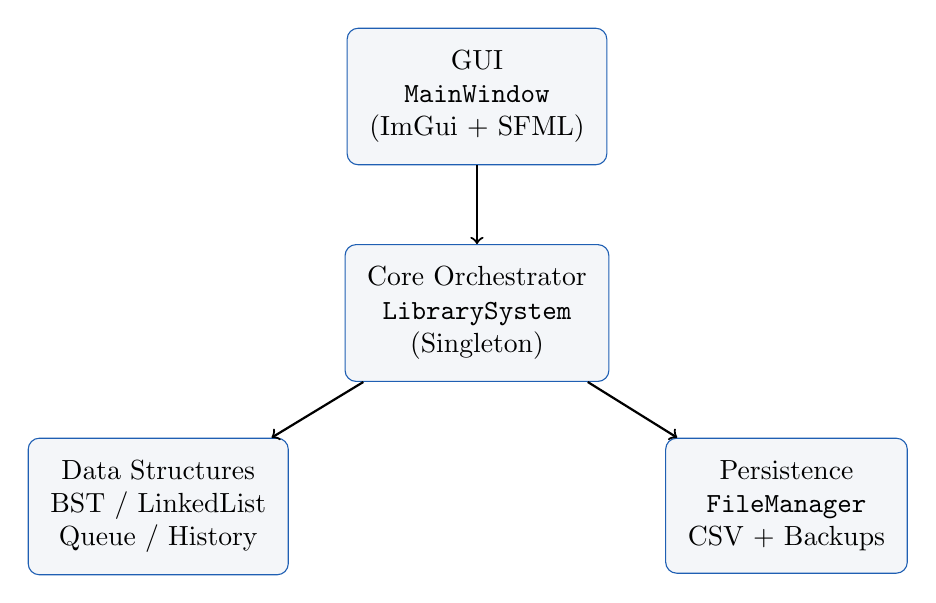
\begin{tikzpicture}[
    node distance=10mm,
    box/.style={draw=AccentBlueDark, rounded corners=4pt, fill=SoftGray, inner sep=8pt, align=center}
  ]
    \node[box] (gui) {GUI\\\texttt{MainWindow}\\(ImGui + SFML)};
    \node[box, below=of gui] (sys) {Core Orchestrator\\\texttt{LibrarySystem}\\(Singleton)};
    \node[box, below left=of sys] (ds) {Data Structures\\BST / LinkedList\\Queue / History};
    \node[box, below right=of sys] (io) {Persistence\\\texttt{FileManager}\\CSV + Backups};

    \draw[->, thick] (gui) -- (sys);
    \draw[->, thick] (sys) -- (ds);
    \draw[->, thick] (sys) -- (io);
  \end{tikzpicture}
  \end{center}
\else
  \begin{infobox}{Architecture (text-only fallback)}
  \begin{itemize}
    \item \textbf{GUI}: \texttt{MainWindow} (Dear ImGui + SFML)
    \item \textbf{Core}: \texttt{LibrarySystem} (singleton orchestrator)
    \item \textbf{Data structures}: BST / LinkedList / Queue / History
    \item \textbf{Persistence}: \texttt{FileManager} (CSV + backups)
  \end{itemize}
  \end{infobox}
\fi

% ----------------------------
% 3. Data Structures
% ----------------------------
\section{Data Structures}
\subsection{BST for Books}
\textbf{Why BST?} Book search by ID is frequent and must be efficient. A BST supports average-case \(O(\log n)\) insert/search/remove.

\begin{itemize}
  \item Key: \texttt{Book::id}
  \item Operations: insert, search(ID), update, remove, traversals, range search
  \item Thread-safety: read-write locking via \texttt{std::shared\_mutex}
\end{itemize}

\subsection{Singly Linked List for Students}
Students are stored in a linked list:
\begin{itemize}
  \item Efficient append, simple iteration, and straightforward serialization.
  \item Thread-safety via \texttt{std::mutex}.
\end{itemize}

\subsection{Circular Queue for Book Requests}
Requests are stored using a circular queue implementation:
\begin{itemize}
  \item FIFO ordering per book.
  \item Operations: enqueue, dequeue, cancel, find position.
\end{itemize}

\subsection{Transaction History (Circular Buffer)}
Transaction history keeps the most recent \(N\) transactions in a fixed-size circular structure:
\begin{itemize}
  \item Fast \(O(1)\) insertion
  \item Supports ``recent transactions'' and student/book filtering
\end{itemize}

% ----------------------------
% 4. Core Workflows
% ----------------------------
\section{Core Workflows}
\subsection{Book Management}
\begin{itemize}
  \item Add book (validation: ID range, non-empty title/author, ISBN-13, quantity \(\ge 1\))
  \item Search by ID (BST), or by Title/Author (linear scan)
  \item Update book info / quantity
  \item Remove book (guarded by system rules)
\end{itemize}

\subsection{Student Management}
\begin{itemize}
  \item Register student (6-digit ID, name/department required, email validated if provided)
  \item Borrowing limit enforced (max 3 active borrows)
  \item Search by ID / name
\end{itemize}

\subsection{Issue / Return}
\begin{itemize}
  \item Issue (Librarian only): verify student exists and can borrow; verify book availability; create transaction; update counts
  \item Return: update book availability; mark transaction returned; compute fine if overdue
  \item When a book becomes available, the system can process waiting requests (queue)
\end{itemize}

\subsection{Authentication and Permissions}
\textbf{Login modes:}
\begin{itemize}
  \item \textbf{Librarian} (admin role): full management privileges.
  \item \textbf{Student}: limited actions, focused on returning and requesting books.
\end{itemize}

\textbf{Policy:}
\begin{itemize}
  \item Librarian can: Add/Edit/Delete books and students; Issue books; Return books; Save/Reload.
  \item Student can: Search/view books; Request books; Return books (for their own ID); use Assistant tab.
\end{itemize}

% ----------------------------
% 5. Persistence
% ----------------------------
\section{Persistence (CSV + Backups)}
Data is stored under \texttt{data/} in CSV form:
\begin{itemize}
  \item \texttt{books.csv}
  \item \texttt{students.csv}
  \item \texttt{transactions.csv}
  \item \texttt{requests.csv}
\end{itemize}

\subsection{CSV Format Notes}
The loader supports:
\begin{itemize}
  \item Header lines (skipped)
  \item Backward compatibility for older \texttt{books.csv} rows
  \item Best-effort loading (bad rows are skipped rather than crashing the app)
\end{itemize}

\subsection{Backups}
Before destructive operations and major saves, backups are created in \texttt{data/backups/}.
This protects against accidental deletes or partial writes.

% ----------------------------
% 6. GUI
% ----------------------------
\section{Graphical User Interface (Dear ImGui + SFML)}
\subsection{Design Goals}
\begin{itemize}
  \item Desktop-app layout: sidebar navigation, content area, status bar
  \item Fast workflows: searchable tables, edit/delete modals, toasts for feedback
  \item Pleasant visuals: light themes with configurable accents
\end{itemize}

\subsection{Screens}
\begin{itemize}
  \item Login: choose Student/Librarian mode and authenticate
  \item Dashboard: overview cards and recent activity preview
  \item Books: search, list, add, edit, delete
  \item Students: search, list, register, delete
  \item Issue/Return: quick forms with feedback
  \item Requests: per-book queues
  \item History/Statistics: tables + dashboard summaries
  \item Student Assistant: offline help + recommendations (Student role)
\end{itemize}

\subsection{Screenshots}
\begin{figure}[h]
  \centering

  % Screenshot paths (kept in resources/screenshots/ for a neat repo)
  \newcommand{\ShotPath}{../../resources/screenshots}

  % Row 1
  \IfFileExists{\ShotPath/dashboard.png}{%
    
\includegraphics[width=0.48\textwidth]{\ShotPath/dashboard.png}%
  }{%
    \fcolorbox{AccentBlueDark}{SoftGray}{\parbox[c][0.18\textheight][c]{0.48\textwidth}{\centering Missing: dashboard.png}}%
  }\hfill
  \IfFileExists{\ShotPath/Books.png}{%
    
\includegraphics[width=0.48\textwidth]{\ShotPath/Books.png}%
  }{%
    \fcolorbox{AccentBlueDark}{SoftGray}{\parbox[c][0.18\textheight][c]{0.48\textwidth}{\centering Missing: Books.png}}%
  }

  \vspace{0.6em}

  % Row 2
  \IfFileExists{\ShotPath/students.png}{%
    
\includegraphics[width=0.48\textwidth]{\ShotPath/students.png}%
  }{%
    \fcolorbox{AccentBlueDark}{SoftGray}{\parbox[c][0.18\textheight][c]{0.48\textwidth}{\centering Missing: students.png}}%
  }\hfill
  \IfFileExists{\ShotPath/issue_return.png}{%
    
\includegraphics[width=0.48\textwidth]{\ShotPath/issue_return.png}%
  }{%
    \fcolorbox{AccentBlueDark}{SoftGray}{\parbox[c][0.18\textheight][c]{0.48\textwidth}{\centering Missing: issue\_return.png}}%
  }

  \vspace{0.6em}

  % Row 3
  \IfFileExists{\ShotPath/request.png}{%
    
\includegraphics[width=0.48\textwidth]{\ShotPath/request.png}%
  }{%
    \fcolorbox{AccentBlueDark}{SoftGray}{\parbox[c][0.18\textheight][c]{0.48\textwidth}{\centering Missing: request.png}}%
  }\hfill
  \IfFileExists{\ShotPath/history.png}{%
    
\includegraphics[width=0.48\textwidth]{\ShotPath/history.png}%
  }{%
    \fcolorbox{AccentBlueDark}{SoftGray}{\parbox[c][0.18\textheight][c]{0.48\textwidth}{\centering Missing: history.png}}%
  }

  \vspace{0.6em}

  % Row 4 (optional)
  \IfFileExists{\ShotPath/statistics.png}{%
    
\includegraphics[width=0.48\textwidth]{\ShotPath/statistics.png}%
  }{%
    \fcolorbox{AccentBlueDark}{SoftGray}{\parbox[c][0.18\textheight][c]{0.48\textwidth}{\centering Missing: statistics.png}}%
  }\hfill
  \IfFileExists{\ShotPath/fill_tab.png}{%
    
\includegraphics[width=0.48\textwidth]{\ShotPath/fill_tab.png}%
  }{%
    \fcolorbox{AccentBlueDark}{SoftGray}{\parbox[c][0.18\textheight][c]{0.48\textwidth}{\centering Missing: fill\_tab.png}}%
  }

  \caption{GUI screenshots: Dashboard, Books, Students, Issue/Return, Requests, History, and Statistics.}
\end{figure}

% ----------------------------
% 7. Build & Run
% ----------------------------
\section{Build, Run, and Test}
\subsection{Build (GUI)}
\begin{lstlisting}
cmake -S . -B build-gui -DCMAKE_BUILD_TYPE=Release
cmake --build build-gui -j 4
./build-gui/library_gui
\end{lstlisting}

\subsection{Login (Demo Credentials)}
\begin{itemize}
  \item Librarian: \texttt{admin / admin123}
  \item Student: \texttt{100001 / 0001}, \texttt{100002 / 0002}
\end{itemize}

PIN rule: last 4 digits of the Student ID (e.g., 100002 $\rightarrow$ 0002).

\section{Team Contributions (8 Members)}
\begin{infobox}{Distribution of Work}
\textbf{Project Manager:} Suliman Naseeri \\
\textbf{Critical sections assigned to:} Muhammad Asif Khan
\end{infobox}

\begin{tabularx}{\textwidth}{>{\bfseries}l X}
\toprule
Member & Responsibilities \\
\midrule
Suliman Naseeri (PM) & Planning, task breakdown, milestones, reviews, coordination, final submission checklist. \\
Muhammad Asif Khan (Critical) & Core integration and correctness: LibrarySystem orchestration, GUI integration, login/roles enforcement, persistence reliability, final build hygiene. \\
Nelorfar Hussain & UI/UX review and consistency: layout polish, theme coherence, accessibility/labels, screenshot preparation. \\
Muneera Omer & Documentation lead: LaTeX report structure, diagrams/flow descriptions, update notes, ensuring docs match implementation. \\
Momina Ali & Testing and QA: unit/integration tests, edge cases (borrow limits, duplicates), regression checks after changes. \\
Muhammad Yousaf & Data structures review: BST/LinkedList/Queue correctness, complexity notes, test scenarios. \\
Dawood Shah & File I/O and data formats: CSV structure verification, backup/restore behavior, data migration/backward-compat checks. \\
Hammad Durrani & Student assistant content and recommendations: refining prompts/responses, improving recommendation heuristics, validating student-only permissions. \\
\bottomrule
\end{tabularx}

\subsection{Tests}
Tests are built as small executables and run via CTest:
\begin{lstlisting}
cmake -S . -B build-tests -DCMAKE_BUILD_TYPE=Debug -DBUILD_TESTS=ON
cmake --build build-tests -j 4
ctest --test-dir build-tests --output-on-failure
\end{lstlisting}

\subsection{Sanitizers (Debug hardening)}
\begin{lstlisting}
cmake -S . -B build-asan -DCMAKE_BUILD_TYPE=Debug -DBUILD_TESTS=ON -DENABLE_SANITIZERS=ON
cmake --build build-asan -j 4
ctest --test-dir build-asan --output-on-failure
\end{lstlisting}

% ----------------------------
% 8. Performance
% ----------------------------
\section{Performance Notes}
\begin{tabularx}{\textwidth}{l X}
\toprule
\textbf{Component} & \textbf{Notes} \\
\midrule
BST (Books) & Average-case \(O(\log n)\) for insert/search/remove; inorder traversal provides sorted listing. \\
LinkedList (Students) & Linear search \(O(n)\), acceptable for moderate student counts. \\
Queue (Requests) & \(O(1)\) enqueue/dequeue; supports cancellation/position lookups. \\
Transaction History & Fixed-size circular buffer with \(O(1)\) add and fast ``recent'' queries. \\
\bottomrule
\end{tabularx}

% ----------------------------
% 9. Conclusion & Future Work
% ----------------------------
\section{Conclusion and Future Work}
This project demonstrates a full end-to-end system: strong domain validation, custom data structures, persistence, and a professional GUI.

\subsection{Future Enhancements}
\begin{itemize}
  \item Richer search (filters, sorting persistence, advanced query UI)
  \item Better reporting (export to PDF/CSV, charts)
  \item Stronger request processing policies (true priority queue)
  \item Improved configuration system (editable \texttt{settings.ini} driving runtime behavior)
\end{itemize}

\end{document}


